% A example template for the baposter class
% nicolas.renet@uni-graz.at
% References:
% + baposter original repo: http://www.brian-amberg.de/uni/poster/
% + baposter github fork: https://github.com/pietvo/baposter/
% + this template github: 
% 10/2025

\documentclass[a0paper,portrait]{baposter}
\usepackage{comment}
\usepackage{multicol}
\usepackage{hyperref} % for \url
\usepackage{lmodern}
\usepackage{lipsum,graphicx}
\usepackage{multirow}
\usepackage[utf8]{inputenc} %unicode support
\usepackage[T1]{fontenc}
\usepackage{enumitem}
\usepackage{setspace}

%\font\nullfont=cmr10


\selectcolormodel{cmyk}

\graphicspath{{pics/}} % Directory in which figures are stored

\newcommand{\compresslist}{
	\setlength{\itemsep}{0pt}%
	\setlength{\parskip}{1pt}%
	\setlength{\parsep}{0pt}%
}

\newenvironment{boenumerate}%
  {\begin{enumerate}\renewcommand\labelenumi{\textbf\theenumi.}}%
  {\end{enumerate}}



\definecolor{ivygreen}{HTML}{B1D1A3}
\definecolor{vanillacream}{HTML}{FFF9B8}
\definecolor{graz_yellow}{HTML}{FFDF00}
\definecolor{graz_gray}{HTML}{666666}
\definecolor{graz_black}{HTML}{000000}

\begin{document}
\begin{poster} % IMPORTANT: no empty lines between poster args { <config }{ <eye-catcher> }{ <title> }{ <authors }{ <uni logo> }
{
grid=false, % helps with the box layout: set to false when happy with it
headerborder=open, % Adds a border around the header of content boxes
colspacing=1em, % Column spacing
bgColorOne=white, % Background color for the gradient on the left (top) of the poster
bgColorTwo=ivygreen, % Background color for the gradient on the right (bottom) of the poster
background=shadetb, % Background gradient {plain,shadelr,shadetb}
borderColor=ivygreen, % Border color
headerColorOne=graz_yellow, % Background color for the header in the content boxes (left side)
headerColorTwo=graz_black, % Background color for the header in the content boxes (right side)
headerFontColor=graz_black, % Text color for the header text in the content boxes
boxColorOne=white, % Background color of the content boxes
textborder=rounded, % Format of the border around content boxes, can be: none, bars, coils, triangles, rectangle, rounded, roundedsmall, roundedright or faded
eyecatcher=true, % Set to false for ignoring the left logo in the title and move the title left
headerheight=0.11\textheight, % Height of the header
headershape=rectangle, % Specify the rounded corner in the content box headers, can be: rectangle, small-rounded, roundedright, roundedleft or rounded
headershade=plain,
headerfont=\Large\textsf, % Large, bold and sans serif font in the headers of content boxes
%textfont={\setlength{\parindent}{1.5em}}, % Uncomment for paragraph indentation
linewidth=2pt % Width of the border lines around content boxes
}
%%% Eye-catcher %%%%%%% only shown if eye-catcher=true %%%%%%%%%%%%%%%%%%%%%%%%
{\begin{minipage}{.125\linewidth}
	
\includegraphics[width=\linewidth]{didip_sm.png}

	
\includegraphics[width=\linewidth]{logo_erc-flag_eu.png}
\end{minipage}}
%%% Title %%%%%%%%%%%%%%%%%%%%%%%%%%%%%%%%%%%%%%%%%%%%%%%%%%%%%%%%%%%%%%%%%%%%%
{
	\textsf{This Is A Rather Long Title For A Digital\\ 
	Humanities Poster Presentation}
}
%%% Authors %%%%%%%%%%%%%%%%%%%%%%%%%%%%%%%%%%%%%%%%%%%%%%%%%%%%%%%%%%%%%%%%%%%
{
\sf\vspace{.2em}
First Author, Second Author\\
\vspace{.2em}
{\small Department of Digital Humanities, University of Graz}
}
% For contributors from different labs:
% {
% \sf\vspace{.2em}\\
% First Author^{1}$, Second Author$^{2}$
% \vspace{.2em}\\
% $^{1}$Department of Digital Humanities, University of Graz\\
% $^{2}$Institute for Machine Learning, TU Graz
% }
%%% University logo %%%%%%%%%%%%%%%%%%%%%%%%%%%%%%%%%%%%%%%%%%%%%%%%%%%%%%%%%%%
{

\includegraphics[width=.125\linewidth]{unigraz_logo.png} % UniGraz logo
}

% this states the box starts at column 0 (edge of page), row 0 (top of page) for a span of 3 (columns wide)
\begin{posterbox}[name=introduction,column=0,row=0, span=3]{Introduction}
	\small
    \lipsum*[19]
	\vspace{1em}

	%\setlist{nolistsep} % makes space above the list tighter
    \begin{minipage}{.48\linewidth}
		\textbf{Challenges:}
		\begin{itemize}
            \compresslist % more compact list items
			\item Ex sapien vitae pellentesque sem placerat in id.
			\item Pretium tellus duis convallis tempus leo eu aenean.
		\end{itemize}
	\end{minipage}%
	\hfill\vline\hfill%
	\begin{minipage}{.48\linewidth}
		\textbf{Constraints:}
		\begin{itemize}
            \compresslist
			\item Montes nascetur ridiculus mus donec rhoncus eros lobortis.
            \item Aenean sed diam urna tempor pulvinar vivamus fringilla. 
			\end{itemize}
	\end{minipage}
\end{posterbox}

% this states the box starts at column 0 (edge of page), directly below the box labelled 'introduction' for a span of 1 (column wide)
\begin{posterbox}[name=pseudo-figure,column=0,below=introduction,span=1]{Pseudo-figures}

	\small
	    
	% the 'figure' environment may not occur in a box; this is a workaround:
        \begin{minipage}{\textwidth}
        \centering
        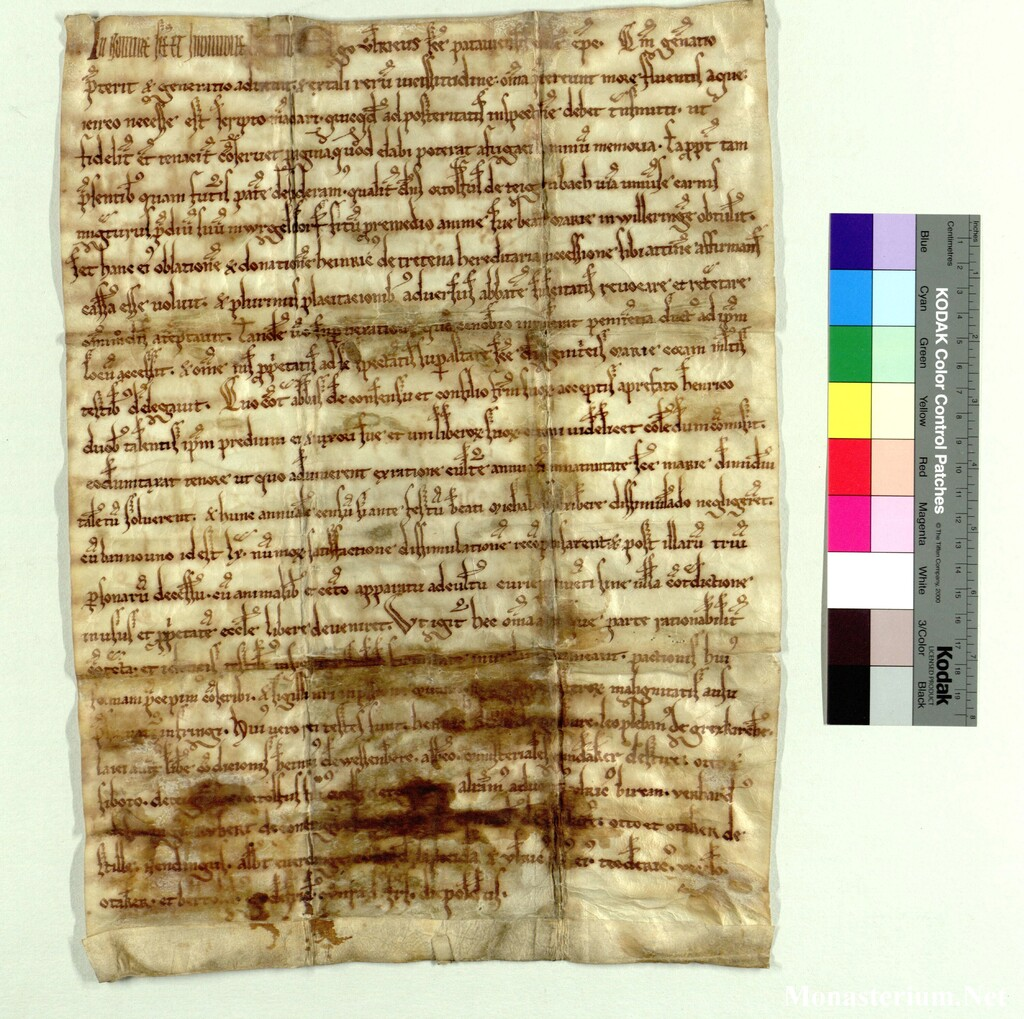
\includegraphics[width=.6\textwidth]{9bde06a84833576b4027ae6331553753.img.jpg}\\
         \vspace{.1em}
         Fig.~1: A charter
        \end{minipage}
        \vspace{1em}
        
        \lipsum*[2][1-5]
\end{posterbox}

\begin{posterbox}[name=pdf-plot,column=1,below=introduction,span=1]{Pdf Plot}
	\lipsum*[5]

	\lipsum*[7][5-8]
\end{posterbox}

\begin{posterbox}[name=vertical-box,column=2,below=introduction]{Vertical span}
\lipsum[10-12]

\lipsum*[1][9-11]
\end{posterbox}



\begin{posterbox}[name=segmentation,column=0,span=2,below=pseudo-figure]{Two-column box, with compact lists}

\begin{multicols}{2}
	A list:
	\begin{itemize}
        \compresslist
		\item Etiam volutpat sem sed felis pulvinar consequat.
		\item In lobortis mi nec nulla dictum, sed interdum sapien scelerisque.
		\item Nam non nulla at lectus rhoncus lacinia.
	\end{itemize}
    \lipsum[1-2]
\end{multicols}

\end{posterbox}

\begin{posterbox}[name=htr,column=0,below=segmentation,span=2,above=bottom]{PDF plots}
	\begin{minipage}{.48\linewidth}
		\lipsum[5]
	\end{minipage}\hfill
	\begin{minipage}{.48\linewidth}
	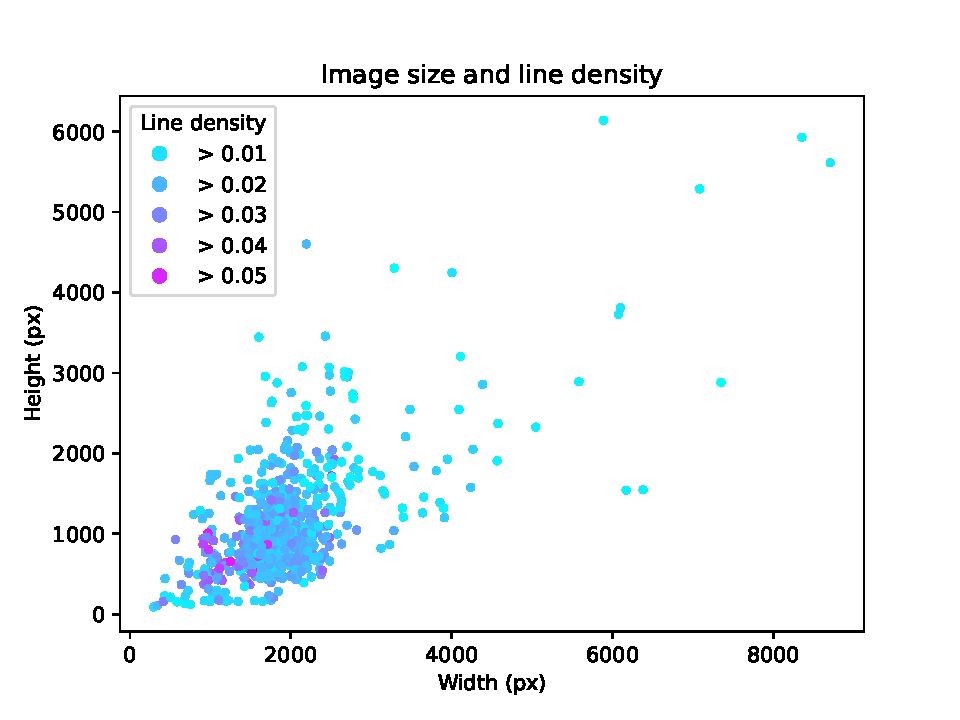
\includegraphics[width=\textwidth]{img_size_scatter_plot.pdf}
	\end{minipage}%
\end{posterbox}



\begin{posterbox}[name=references,column=2,below=segmentation,span=1,above=bottom,headerColorOne=white]{References}

	Brian {\sc Amberg}, original code for \texttt{baposter}:  \url{http://www.brian-amberg.de/uni/poster/}
	\vspace{2em}

	Pieter {\sc van Oostrum}, \texttt{baposter} fork: \url{https://github.com/pietvo/baposter}


\vspace{2em}
\centering
\begin{tabular}{cc}

\includegraphics[width=2.1cm]{qr_monasterium.png} &
	
\includegraphics[width=2.1cm]{qr_didip.png} \\
Monasterium & 
	DiDip
\end{tabular}
\end{posterbox}


\end{poster}

\end{document}
